\documentclass[a4paper,11pt]{article}
\usepackage[T1]{fontenc}
\usepackage[utf8]{inputenc}
\usepackage[english]{babel}
\usepackage{amsmath,amssymb,mathtools}
\usepackage[margin=2.2cm]{geometry}
\usepackage{xcolor,tikz}
\usepackage{booktabs}
\usepackage[most]{tcolorbox}
\setlength{\parindent}{0pt}
\setlength{\parskip}{4pt}
\allowdisplaybreaks
\providecommand{\explainmode}{0}
\newif\ifexplain
\ifnum\explainmode=1 \explaintrue\fi
\newcommand{\aufgabe}[1]{\section*{#1}}
\newcommand{\angabe}[1]{\textit{#1}\par\smallskip}
\newcommand{\teil}[1]{\subsection*{#1}}
\newcommand{\why}[1]{\text{\small\color{black!65}#1}}
\newtcolorbox{erklbox}{colback=blue!4,colframe=blue!40,breakable,boxrule=0.5pt,title={Erklärung}}
\newcommand{\explain}[1]{\ifexplain\begin{erklbox}#1\end{erklbox}\fi}
\newcommand{\explainfig}[1]{\ifexplain\begin{center}#1\end{center}\fi}
\begin{document}
\begin{center}
{\Large Exercise sheet 8}\\
Linear Optimization (311.160), WS 2026/27\\
Raphael Bleier \qquad 23 November 2026
\end{center}

\explain{Dieses Blatt dreht sich um die Dualisierung. Zuerst wird begründet, warum die rot markierten Zeilen des Dualisierungsrezepts gelten. Danach zeigt Aufgabe 8.1, dass primales und duales Problem gleichzeitig unzulässig sein können, und wie eine einzige Zusatznebenbedingung das duale Problem zulässig und unbeschränkt macht. Aufgabe 8.2 überträgt das Rezept auf Minimierungsprobleme, Aufgabe 8.3 zeigt, dass zweimaliges Dualisieren wieder das Ausgangsproblem liefert und dass die schwache Dualität dabei unverändert bleibt.}

\explain{Classroom task 8.1, nur als Lernzusatz, nicht Teil der Abgabe. Die Tabelle gibt das Dualisierungsrezept für ein Maximierungsproblem an. Begründet wurden in der Vorlesung nur die schwarzen Zeilen: eine $\le$-Nebenbedingung erzeugt eine nichtnegative duale Variable, eine Gleichung eine freie duale Variable, und eine nichtnegative primale Variable erzeugt eine $\ge$-Dualnebenbedingung. Die roten Teile lassen sich alle auf genau diese drei Regeln zurückführen.}

\explain{$(Ax)_i\ge b_i \Rightarrow y_i\le 0$: Man multipliziert die $\ge$-Nebenbedingung mit $-1$. Dann steht $-(Ax)_i\le -b_i$ da, also eine $\le$-Nebenbedingung. Deren duale Variable nennen wir $y_i'$, sie ist nach der bekannten Regel $\ge 0$. Die duale Variable des Rezepts gehört aber zur ursprünglichen Nebenbedingung, also ist $y_i=-y_i'\le 0$. Das Minus ist nur eine Umbenennung, am dualen Problem ändert sich sonst nichts.}

\explain{$x_j$ frei $\Rightarrow (A^Ty)_j=c_j$: Eine freie Variable schreibt man als Differenz zweier nichtnegativer Variablen, $x_j=x_j^+-x_j^-$ mit $x_j^+,x_j^-\ge0$. Die schwarze Regel für nichtnegative Variablen liefert dann zwei Dualnebenbedingungen: $(A^Ty)_j\ge c_j$ für $x_j^+$ und $-(A^Ty)_j\ge -c_j$ für $x_j^-$. Die zweite ist äquivalent zu $(A^Ty)_j\le c_j$. Zusammen ergeben die beiden Ungleichungen die Gleichheit $(A^Ty)_j=c_j$.}

\explain{$x_j\le0 \Rightarrow (A^Ty)_j\le c_j$: Man setzt $x_j=-x_j'$ mit $x_j'\ge0$. In der Matrix $A$ wird dadurch die Spalte $j$ durch $-a_j$ ersetzt und in $c$ der Eintrag $c_j$ durch $-c_j$. Die schwarze Regel für die nichtnegative Variable $x_j'$ verlangt dann $(-a_j)^Ty\ge -c_j$, also $(A^Ty)_j\le c_j$.}

\aufgabe{Exercise 8.1 (An infeasible problem with infeasible dual problem)}
\angabe{In this exercise we will see that it is possible that both the primal and its dual problem are infeasible. Consider the LP
\[
\text{maximize } 2x_1 - x_2 \quad\text{subject to}\quad x_1 - x_2 \le 1,\quad -x_1 + x_2 \le -2,\quad x_1, x_2 \ge 0.
\]
1. Show graphically that the program is infeasible. 2. Determine the dual LP and use the previous result to show that it is infeasible as well. 3. Add a constraint to the primal problem such that the dual problem becomes feasible and unbounded.}

\teil{1. The primal is infeasible}
Rewrite each constraint so that $x_2$ is isolated:
\begin{align*}
x_1 - x_2 &\le 1 && \why{first constraint}\\
-x_2 &\le 1 - x_1 && \why{$|\,-x_1$}\\
x_2 &\ge x_1 - 1 && \why{$|\,\cdot(-1)$}\\
-x_1 + x_2 &\le -2 && \why{second constraint}\\
x_2 &\le x_1 - 2 && \why{$|\,+x_1$}
\end{align*}
A feasible point would have to satisfy $x_1 - 1 \le x_2 \le x_1 - 2$, which needs $x_1 - 1 \le x_1 - 2$, that is $-1 \le -2$. That is impossible, so no feasible point exists.
\explain{Beide Grenzen sind Geraden mit Steigung $1$, also parallel. Die erste Nebenbedingung verlangt den Bereich oberhalb der Geraden $x_2=x_1-1$, die zweite den Bereich unterhalb der Geraden $x_2=x_1-2$. Die Gerade $x_2=x_1-1$ liegt immer über der Geraden $x_2=x_1-2$, deshalb überschneiden sich die beiden Halbebenen nirgends. Die Nichtnegativität $x_1,x_2\ge0$ macht das nicht besser: Der Widerspruch entsteht schon allein aus den beiden Ungleichungen.}
\begin{center}
% grafik-verlangt
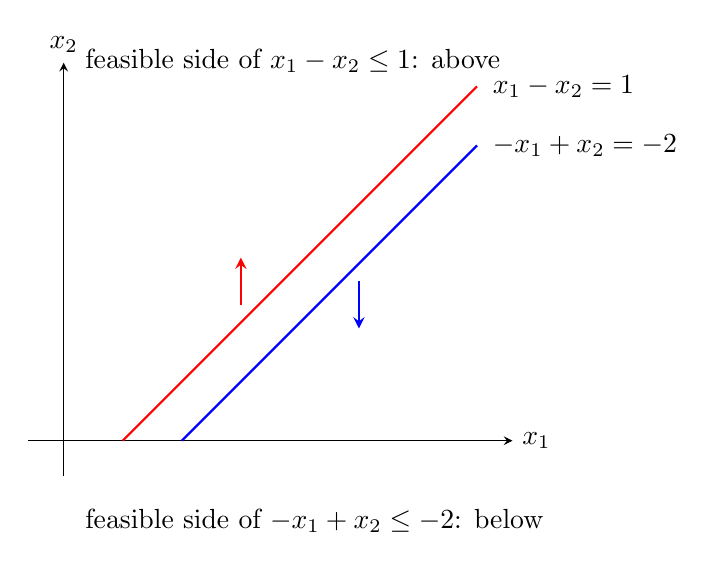
\begin{tikzpicture}[scale=0.75, >=stealth]
  \draw[->] (-0.6,0)--(7.6,0) node[right]{$x_1$};
  \draw[->] (0,-0.6)--(0,6.4) node[above]{$x_2$};
  \draw[thick,red] (1,0)--(7,6) node[right=2pt,black]{$x_1-x_2=1$};
  \draw[thick,blue] (2,0)--(7,5) node[right=2pt,black]{$-x_1+x_2=-2$};
  \draw[->,red,thick] (3,2.3)--(3,3.1);
  \draw[->,blue,thick] (5,2.7)--(5,1.9);
  \node[anchor=north west] at (0.2,6.8) {feasible side of $x_1-x_2\le1$: above};
  \node[anchor=north west] at (0.2,-1.0) {feasible side of $-x_1+x_2\le-2$: below};
\end{tikzpicture}
\end{center}
The two half-planes point away from each other, so the feasible region is empty.
\explain{Die rote Gerade ist $x_2=x_1-1$, die blaue $x_2=x_1-2$. Der rote Pfeil zeigt in die zulässige Richtung der ersten Nebenbedingung (nach oben, $x_2\ge x_1-1$), der blaue in die der zweiten (nach unten, $x_2\le x_1-2$). Beide Pfeile zeigen voneinander weg.}
Adding the two constraints gives the contradiction algebraically as well:
\begin{align*}
(x_1 - x_2) + (-x_1 + x_2) &\le 1 + (-2) && \why{add the two constraints}\\
0 &\le -1 && \why{collect terms}
\end{align*}
\[
\boxed{\text{primal infeasible}}
\]

\teil{2. The dual is infeasible as well}
Write the primal as $\max c^Tx$ s.t. $Ax\le b$, $x\ge0$ with
\[
A = \begin{pmatrix}1&-1\\-1&1\end{pmatrix},\qquad b=\begin{pmatrix}1\\-2\end{pmatrix},\qquad c=\begin{pmatrix}2\\-1\end{pmatrix}.
\]
\explain{Die Dualisierung tauscht die Rollen: Aus $A$ wird $A^T$, aus $b$ wird die duale Zielfunktion, aus $c$ die rechte Seite der dualen Nebenbedingungen. Weil alle primalen Nebenbedingungen $\le$ sind, werden alle dualen Variablen $\ge0$; weil $x\ge0$ gilt, werden alle dualen Nebenbedingungen $\ge$.}
By the dualization recipe ($\le$ constraint $\Rightarrow y_i\ge0$, $x_j\ge0 \Rightarrow (A^Ty)_j\ge c_j$) the dual is $\min b^Ty$ s.t. $A^Ty\ge c$, $y\ge0$:
\begin{align*}
\min\;& y_1 - 2y_2 && \why{$b=(1,-2)^T$}\\
\text{s.t.}\;& y_1 - y_2 \ge 2 && \why{column 1 of $A$: $(A^Ty)_1 \ge c_1 = 2$}\\
& -y_1 + y_2 \ge -1 && \why{column 2 of $A$: $(A^Ty)_2 \ge c_2 = -1$}\\
& y_1, y_2 \ge 0 && \why{primal constraints are $\le$}
\end{align*}
The two dual constraints say $y_1-y_2\ge2$ and $y_1-y_2\le1$. Reordering them and setting $(x_1,x_2)=(y_1,y_2)$ gives the same two half-planes as in part 1. Hence the dual is infeasible by the same graph. Adding the two dual constraints also checks this algebraically:
\begin{align*}
(y_1 - y_2) + (-y_1 + y_2) &\ge 2 + (-1) && \why{add the two constraints}\\
0 &\ge 1 && \why{collect terms}
\end{align*}
This is impossible, so the dual is infeasible.
\[
\boxed{\text{dual infeasible}}
\]
\explain{Dasselbe Argument wie beim Primalen, nur mit vertauschten Zahlen: Die beiden dualen Nebenbedingungen sind $y_1-y_2\ge2$ und $y_1-y_2\le1$. Sie widersprechen sich genauso wie vorher $x_1-x_2\le1$ und $x_1-x_2\ge2$.}

\teil{3. Making the dual feasible and unbounded}
Add the constraint $x_1 \le -1$ to the primal. The primal stays infeasible, because it already requires $x_1 \ge 0$. The new data are
\[
A = \begin{pmatrix}1&-1\\-1&1\\1&0\end{pmatrix},\qquad b=\begin{pmatrix}1\\-2\\-1\end{pmatrix},\qquad c=\begin{pmatrix}2\\-1\end{pmatrix}.
\]
The dual now has three variables, one per constraint:
\begin{align*}
\min\;& y_1 - 2y_2 - y_3 && \why{$b=(1,-2,-1)^T$}\\
\text{s.t.}\;& y_1 - y_2 + y_3 \ge 2 && \why{column 1 of $A$: $(A^Ty)_1 \ge c_1 = 2$}\\
& -y_1 + y_2 \ge -1 && \why{column 2 of $A$: $(A^Ty)_2 \ge c_2 = -1$}\\
& y_1, y_2, y_3 \ge 0 && \why{primal constraints are $\le$}
\end{align*}
\explain{Die dritte Nebenbedingung $x_1\le-1$ bringt eine dritte duale Variable $y_3\ge0$ mit dem Koeffizienten $-1$ in der Zielfunktion und der Spalte $(1,0)^T$ in $A^T$. Dadurch bekommt die erste duale Nebenbedingung den Zusatzterm $+y_3$, der sie erfüllbar macht.}
Feasibility: the point $y=(0,0,2)$ works:
\begin{align*}
y_1 - y_2 + y_3 &= 0 - 0 + 2 && \why{substitute $y=(0,0,2)$}\\
&= 2 && \why{$0-0+2=2$}\\
2 &\ge 2 && \why{first constraint: right-hand side $c_1=2$}\\
-y_1 + y_2 &= -0 + 0 && \why{substitute $y=(0,0,2)$}\\
&= 0 && \why{$-0+0=0$}\\
0 &\ge -1 && \why{second constraint: right-hand side $c_2=-1$}
\end{align*}
So the dual is feasible.
\explain{Der Punkt $(0,0,2)$ macht genau die erste Nebenbedingung scharf: $y_3=2$ gleicht aus, dass $y_1-y_2=0$ ist. Die zweite Nebenbedingung ist mit $0\ge-1$ locker erfüllt.}
Unboundedness: from this feasible point, $y_3$ can grow arbitrarily. For any $t \ge 0$, set $y(t)=(0,0,2+t)$. Its constraints stay valid:
\begin{align*}
y_1 - y_2 + y_3 &= 0 - 0 + (2+t) && \why{substitute $y(t)$}\\
&= 2 + t && \why{simplify}\\
2 + t &\ge 2 && \why{$t \ge 0$}\\
-y_1 + y_2 &= 0 && \why{substitute $y(t)$}\\
0 &\ge -1 && \why{second constraint: right-hand side $c_2=-1$}
\end{align*}
The objective along this ray is
\begin{align*}
y_1 - 2y_2 - y_3 &= 0 - 0 - (2+t) && \why{substitute $y(t)$}\\
&= -2 - t && \why{simplify}\\
&\to -\infty && \why{$t\to\infty$}
\end{align*}
Since the dual is a minimization and its objective can be made arbitrarily small, it is unbounded.
\[
\boxed{\text{with } x_1 \le -1:\ \text{the dual is feasible and unbounded}}
\]
\explain{Der Strahl $y(t)=(0,0,2+t)$ bleibt zulässig, weil $y_3$ nur in der ersten Nebenbedingung mit positivem Vorzeichen vorkommt und deren linke Seite damit nur größer wird. Die zweite Nebenbedingung hängt gar nicht von $y_3$ ab. In der Zielfunktion steht $y_3$ mit Koeffizient $-1$, also fällt der Wert bei wachsendem $t$ gegen $-\infty$.}

\aufgabe{Exercise 8.2 (The dual problem of a minimization problem)}
\angabe{Consider the dualization recipe for a maximization problem of the lecture notes and write the same recipe for a minimization problem. In particular, the last step consists of filling the following table:
\begin{center}
\begin{tabular}{@{}llll@{}}
\toprule
Primal constraint & Dual variable sign & Primal variable sign & Dual constraint\\
\midrule
$(Ax)_i\le b_i$ & & $x_j\ge0$ & \\
$(Ax)_i=b_i$ & & $x_j$ free & \\
$(Ax)_i\ge b_i$ & & $x_j\le0$ & \\
\bottomrule
\end{tabular}
\end{center}}

\teil{The recipe for minimization}
A minimization problem becomes a maximization problem by negating the objective:
\[
\min c^Tx = -\max(-c^Tx).
\]
\explain{Minimieren und Maximieren hängen über das Vorzeichen zusammen: Den kleinsten Wert von $f$ zu finden ist dasselbe, wie den größten Wert von $-f$ zu finden und davon das Vorzeichen zu nehmen. Deshalb kann man das Rezept für Maximierungsprobleme wiederverwenden.}
Apply the maximization recipe to $\max(-c^Tx)$ with the same constraints and variable signs. It produces a minimization in a variable $z$; the substitution $y=-z$ then turns it back into a maximization.
\explain{Warum die Substitution $y=-z$? Das Rezept für $\max(-c^Tx)$ liefert ein Minimierungsproblem in $z$. Das duale Problem eines Minimierungsproblems soll aber ein Maximierungsproblem sein. Mit $y=-z$ dreht man das Vorzeichen der Zielfunktion um, aus $\min b^Tz$ wird $\max b^Ty$.}
\begin{center}
\begin{tabular}{@{}lll@{}}
\toprule
primal form & recipe on $\max(-c^Tx)$ (variable $z$) & set $y=-z$\\
\midrule
$(Ax)_i\le b_i$ & $z_i\ge0$ & $y_i\le0$\\
$(Ax)_i=b_i$ & $z_i$ free & $y_i$ free\\
$(Ax)_i\ge b_i$ & $z_i\le0$ & $y_i\ge0$\\
$x_j\ge0$ & $(A^Tz)_j\ge -c_j$ & $(A^Ty)_j\le c_j$\\
$x_j$ free & $(A^Tz)_j=-c_j$ & $(A^Ty)_j=c_j$\\
$x_j\le0$ & $(A^Tz)_j\le -c_j$ & $(A^Ty)_j\ge c_j$\\
\bottomrule
\end{tabular}
\end{center}
\explain{In der mittleren Spalte steht wörtlich das Rezept für Maximierungsprobleme, nur mit $-c$ statt $c$ als Zielfunktionsvektor. Die rechte Spalte entsteht daraus mit $y=-z$: Jede Ungleichung mit $-c$ wird mit $-1$ durchmultipliziert, dadurch drehen sich die Relationszeichen um.}
The dual of a minimization problem is therefore a maximization problem $\max b^Ty$, and the filled table reads
\begin{center}
\begin{tabular}{@{}llll@{}}
\toprule
Primal constraint & Dual variable sign & Primal variable sign & Dual constraint\\
\midrule
$(Ax)_i\le b_i$ & $y_i\le0$ & $x_j\ge0$ & $(A^Ty)_j\le c_j$\\
$(Ax)_i=b_i$ & $y_i$ free & $x_j$ free & $(A^Ty)_j=c_j$\\
$(Ax)_i\ge b_i$ & $y_i\ge0$ & $x_j\le0$ & $(A^Ty)_j\ge c_j$\\
\bottomrule
\end{tabular}
\end{center}
\explain{Kurz gemerkt: Gegenüber dem Maximierungsrezept drehen sich in der Dualisierung eines Minimierungsproblems alle Ungleichheitszeichen um. Eine $\ge$-Nebenbedingung wird zur nichtnegativen dualen Variable, eine nichtnegative Variable zur $\le$-Dualnebenbedingung.}
\[
\boxed{\min c^Tx \ \Longleftrightarrow\ \max b^Ty}
\]

\aufgabe{Exercise 8.3 (The dual of the dual)}
\angabe{Consider the maximization problem
\[
(P)\qquad \max c^Tx \quad\text{s.t.}\quad Ax \le b,\quad x \ge 0,
\]
and call its dual (D). 1. Show that dualizing twice returns the original problem, i.e., the dual of (D) is (P). 2. State weak duality for (D) (considered as primal problem) and (P) (considered as dual problem). What do you notice?}

\teil{1. The dual of the dual}
By the maximization recipe ($\le$ constraint $\Rightarrow y_i\ge0$, $x_j\ge0 \Rightarrow (A^Ty)_j\ge c_j$), the dual of (P) is
\[
(D)\qquad \min b^Ty \quad\text{s.t.}\quad A^Ty \ge c,\quad y \ge 0.
\]
\explain{(D) ist ein Minimierungsproblem. Seine Matrix ist $A^T$, seine rechte Seite ist $c$, seine Zielfunktionskoeffizienten sind $b$. Zum zweiten Dualisieren braucht man deshalb das Minimierungsrezept aus Aufgabe 8.2.}
Now dualize (D) with the minimization recipe of Exercise 8.2. The constraint $(A^Ty)_j\ge c_j$ is a $\ge$ constraint, so it produces a nonnegative dual variable $z_j\ge0$. The variable sign $y_i\ge0$ produces a $\le$ constraint, namely $((A^T)^Tz)_i\le b_i$, that is $(Az)_i\le b_i$, because $(A^T)^T=A$ and the objective coefficients of (D) are $b$. The dual of (D) is therefore
\[
\max c^Tz \quad\text{s.t.}\quad Az \le b,\quad z \ge 0,
\]
which is exactly (P) with $z$ renamed to $x$.
\[
\boxed{\text{the dual of (D) is (P)}}
\]
\explain{Jede Dualisierung tauscht Zielfunktion und rechte Seite und transponiert die Matrix. Zweimal angewendet heben sich Transponieren und Rollentausch gegenseitig auf: Aus $A$ wird über $A^T$ wieder $A$, aus $b$ über $c$ wieder $b$, aus $c$ über $b$ wieder $c$. Das Vorzeichen der Ungleichungen dreht sich zweimal und landet wieder bei $\le$.}

\teil{2. Weak duality in both directions}
For (P) as the primal (maximization) and (D) as its dual (minimization), weak duality (Theorem 3.3) states: for every feasible $x$ and every feasible $y$,
\[
c^Tx \le b^Ty.
\]
Now consider (D) as the primal (minimization) and (P) as its dual (maximization). Weak duality for this pair states: the primal objective is never below the dual objective, that is, for every feasible $y$ and every feasible $x$,
\[
b^Ty \ge c^Tx.
\]
These two lines say the same thing:
\[
\boxed{c^Tx \le b^Ty \iff b^Ty \ge c^Tx}
\]
What one notices: weak duality is symmetric. Swapping the roles of primal and dual leaves the weak-duality inequality unchanged, only its two sides are exchanged.
\explain{Beim Maximieren gilt für das primale (max) und das duale (min) Problem: primärer Wert $\le$ dualer Wert. Betrachtet man stattdessen das Minimierungsproblem als primal und das Maximierungsproblem als dual, lautet die Regel: primärer (min) Wert $\ge$ dualer (max) Wert. Das ist dieselbe Ungleichung $c^Tx\le b^Ty$, nur von der anderen Seite gelesen.}

\end{document}
